
\section{Instrument response} 
\label{sect:inst-resp}

In SEISAN the instrument response can be stored as pairs of frequency, 
amplitude and phase or as poles and zeros. The formats that can be 
used include GSE2, SEISAN, SAC and SEED. The SEISAN, SAC and GSE response formats 
are described in Appendix \ref{app:response}. For a detailed description of the GSE 
format, the reader is referred to \citet{gsett1997}. The program RESP 
creates response files in SEISAN and GSE format. SEED format response 
files can be extracted from a SEED volume.  

\subsection{Create instrument response files, RESP} 
\index{RESP}\index{Instrument response} 

\textbf{Introduction}

The purpose of this program is to (1) Make Seisan or GSE2 response files, (2) Provide the engineer maintaining seismic instrumentation with a practical tool for calculating and checking response functions of the most common elements of a seismic system. The program can calculate response functions of velocity transducers, accelerometers, filters and amplifiers, input poles and zeros or tabulated values and multiply the combinations together to get complete system response functions. The program produces a table with the response function and a simple graphical expression of the response curve. For the purpose of checking measured values, a file with these values can be used as input and will be plotted together with the theoretical values. The program can calculate, acceleration, velocity or displacement response. Program PR\_ RESP \index{PR\_RESP} can make a table of many response files. 

\textbf{The instrument response}

The seismic recording system can consist of seismic sensor, analog-digital converter, amplifier and filters. For a detailed discussion the user is referred to \citet{scherbaum1996}. The combined response can be given in the frequency domain as frequency response function or in the Laplace domain as transfer function. The frequency response is given in pairs of frequency amplitude phase (FAP), while the transfer function is given as poles and zeros (PAZ). The combined frequency response is obtained through multiplication of the response from the individual components, while the transfer function is obtained by combing the PAZ from the components. Amplifiers and accelerometers are specified simply by a constant gain. Filters are assumed to be Butterworth. RESP can be used to write finite impulse response (FIR) coefficients \citep{scherbaum1996} that are used as anti-alias filters in most modern digitizers if GSE is used as output format. SEISAN has no capability to read the FIR filters or to correct for them. However, the FIR filters are part of a full description of the instrument response and should be at least included for information if possible. 

The electrodynamic seismometer is assumed to have the following velocity frequency response: 

\begin{displaymath}
T(\omega) = \frac{\omega^{2}}{\omega_{0}^2 - \omega^2 + i 2 \omega \omega_0 h}
\end{displaymath}

which corresponds to the transfer function: 

\begin{displaymath}
T(s) = \frac{-s^{2}}{\omega_{0}^2 + s^2 + 2 s \omega_0 h}
\end{displaymath}

where $s=i\omega$, $\omega$ is the angular frequency $2\pi f$ in Hz, $\omega_0$ the 
resonance frequency of the seismometer, $i = \sqrt{-1}$ 
and $h$ the damping (normally around 0.7). 

NOTE: In the equation for the frequency response, the sign "+ 2*i*h.." was "-" before March 2000, so old parameter files may have to be regenerated.\index{Problem, RESP} The sign depends on the definition of the signs in the Fourier transform and therefore may be different  in different text books. It may even be wrong although it looks right, if a wrong Ansatz is done. Due to the wrong sign, the FAP values in the SEISAN response files were wrong, however the programs use the constants given in the files and the correct response is generated. If you have the instrument constants in your old response files and not just FAP, the old response files can be used. 

The transformation from displacement to velocity or back is done by multiplying  with i*.. 

In addition to or instead of using the equation above, values can also be entered as discrete values or as poles and zeros. 

The SEISAN response function is calculated for 60 frequencies between 0.01 and 100 Hz and the steps between the frequencies are approximately logarithmic. The response function is normalised at 
1.0 Hz ( see Table 1) and the gain at 1.0 Hz is given separately.  

NOTE: ALL UNITS ARE IN METERS, SECONDS OR G (9.8ms-2) \index{Units} 

\textbf{NOTE}: It seems that although the GSE format is clearly defined, there 
has been different interpretations. This has also led to changes in 
SEISAN since the GSE response was introduced with SEISAN. For more 
details, see Appendix \ref{app:response}. 

\textbf{Which format to use}

SEISAN, since version 7.1, supports the GSE2 calibration format in addition to the SEISAN response file format. We recommend that you use the GSE2 format, since it presents one of the most widely used calibration formats. Storage of the response in terms of PAZ is recommended over FAP, since the PAZ representation describes the continuous transfer function. You may continue using existing SEISAN response files and add new files in GSE2 format, or replace the old SEISAN response files with new GSE2 files. 

\textbf{How to run the program}

The program has quite a few options, which easily may lead to confusion. Before you start you should know which format you want to use (GSE2 or SEISAN) and whether you want to describe the response in terms of FAP or PAZ. The recommended choice is to use GSE2 and PAZ. 

Type RESP to start the program. You will then get a series of questions as indicated below in upper case letters. All input is format free. A sample run is shown below. 

CHOSE OUTPUT FORMAT: \verb|     |0: NO OUTPUT FILE \newline
\verb|                               |1: SEISAN FAP \newline
\verb|                               |2: SEISAN PAZ \newline
\verb|                               |3: GSE2 FAP \newline
\verb|                               |4: GSE2 PAZ 

Answer with 0-4, options 1-4 will create respective response files in selected format, option 0 will only calculate and show the response on the screen. SEISAN PAZ can only be used if number of poles and number of zeros are less than 38. If more are input, a table will be generated automatically in FAP format. A format with poles and zeros MUST BE USED if a mechnical displacment sensor is selectedor an accelerometer is selected which does not have first character A in component name (see later). 

TYPE OF SENSOR: \verb|      |1: NONE \newline
\verb|                         |2: SEISMOMETER \newline
\verb|                         |3: ACCELEROMETER 
\verb|                         |4: MECHANICAL DISPLACEMENT SEISMOMETER 

Answer with 1, 2, 3 or 4. Number 1 is used when only calculation of filters or amplifiers are desired, 2 is a standard velocity transduceri,  3 a standard accelerometer and 4 is a mechnical diplacement sensor (normally a digitized record of a paper seismogram). If a seismic sensor is used, you will get additional questions on the constants of the sensor. If a seismometer is chosen, the following questions must be answered: 

SEISMOMETER NATURAL PERIOD ? 

This is measured in seconds. For most short period systems the value would be 1.0 second. 

SEISMOMETER DAMPING RATIO ? 

The damping ratio should ideally be 0.7. This depends on the damping resistance. 

For both the electrodynamic seismometer and accelerometer, the following question is given: 

SENSOR LOADED GENERATOR CONSTANT (V/M/S OR V/G) ? 

This is the generator constant of the sensor in terms of volt per unit of of ground motion (meter/second or g). It is important to note that this is the loaded constant, which means the effective output of the sensor taking into account amplifier input and damping resistances.\index{Seismometer constants} 

For the mechanical sensor, the question is

 SEISMOGRAPH GAIN in TIMES GAIN (M/M) ?

which is simply the mechnical gain.

Now comes questions about amplifier, filter and recording unit. 

RECORDING MEDIA GAIN (COUNT/V OR M/V) ? 

If you have a recording media, the gain can be given here, otherwise just enter 1.0 

If the output format is GSE, the response is always calculated in displacement units, while for SEISAN output and seismometer or accelerometer, the following options appear: 

TYPE OF RESPONSE: \verb|    |1: DISPLACEMENT \newline
\verb|                         |2: VELOCITY \newline
\verb|                         |3: ACCELERATION 

Normally for a seismometer, one wants to calculate the displacement response and for an accelerometer, the acceleration response. However it might sometimes be interesting to look at e.g. 
the velocity response for a seismometer (after all, the seismometer is normally a velocity transducer !!). Enter the appropriate number. 

AMPLIFIER GAIN (DB) ? 

This is the amplifier gain in dB. Since this question is only asked once, this gain must include gain of all units except the recorder (asked below). This could e.g. include gain of the VCO system. 

NUMBER OF FILTERS (0-10), RETURN FOR NONE ? 

Up to 10 filters can be specified. If you answer 0, no filters are used and no more questions on filters will appear. Otherwise one line of input must be given for each filter as follows: 

FREQUENCY AND NUMBER OF POLES FOR EACH FILTER, \newline
POLES NEGATIVE FOR HIGH PASS 

Each line requires two numbers, the corner frequency of the filter and the number of poles. A high pass filter is given by letting number of poles be negative. It is not always easy to know whether a filter is e.g. one 2 pole or two 1 pole filters, the user needs to experiment with this. 

FILE NAME FOR FILE WITH POLES AND ZEROS, RETURN FOR NO FILE
\index{Poles and zeros}

Here a file with poles and zeros can be entered. If seismometer constants have been chosen above, the values calculated with poles and zeros are multiplied with the values previously calculated. The free format file contains: 

1. line: NP: Number of poles, NZ: Number of zeros, Norm: Normalization constant \newline
Following NP lines contain one pair each of real and imaginary poles \newline
Following NZ lines contain one pair each of real and imaginary zeros 

NOTE: The unit of frequency is radian/s so if in Hz, multiply with 
$2\pi$ and normalization constant in 
$radian = (normalization constant in Hz) 2\pi^{(number of poles-number of zeroes)}$. 

The next 2 options are only shown if the output file is selected to be FAP: 

FILE NAME FOR TABULATED VALUES, RETURN FOR NO FILE  

Here a file with tabulated values are entered. If seismometer constants or poles and zeros have been chosen above, the tabulated values will be interpolated and multiplied with the values previously calculated for from above. The free format file contains: 

1. line: N: Number of tabulated values, Norm: Normalization constant \newline
Following N lines contain one each frequancy, amplitude and phase(deg) 

GIVE FILE NAME FOR MEASURED VALUES, RETURN FOR NONE 

Give file name for measured values. In most cases you have none so just make a return. The format of the input file is as follows: 

frequency, amplitude, phase \newline
frequency, amplitude, phase \newline
etc. 

e.g. 

0.2,0.7,200 \newline
0.7,0.8,100 \newline
10.0,0.1,33 

The file has no blank lines and can contain up to 60 data sets. It is important to note that the amplitude values should be NORMALIZED at 1.0 Hz. 

Now there is no more input to the response parameters, and the output is: 

GAIN FACTOR AT 1.0 HZ: 12345.6 

This is the gain of the system at 1.0 Hz and is also the value for normalizing the response curve, that is, all calculated values are divided by this number. There is no unit for gain of an amplifier and for displacement response using a seismometer and drum recording. If the recording is digital, the unit would be counts/meter and for a velocity response counts/meter/second etc. If a file with poles and zeros is used without any other information, the \index{Normalization constant}normalization constant must have the unit of count/m, similar for the tabulated input. 

Further output is given in a file called resp.out, see Table 1 for an example. 

The response curves (amplitude and phase) are now printed/plotted on the screen. First comes the amplitude response (amplitude in db versus log frequency). By pushing return, the phase response is shown (phase shift (deg) versus log frequency). After the plots, the SEISAN \index{Calibration file}calibration file can optionally be made, follow instructions, see example below. The response file MUST be calculated for the displacement response, and all calculation in SEISAN assume that response is calculated in counts/m. 

After the SEISAN response file is made, the current parameters will be displayed and one or several can be changed without entering all again. Like if the gain has changed at a certain date, only change date and gain. This feature (new in SEISAN7.2) has been put in to be able to quickly make many similar response files, like when all files have to be put in for a network. 

\textbf{Comments to data for response files}

\index{Station and channel codes}
Station and channel codes \newline
It is important that the station and channel codes are made exactly as they appear in the waveform files. If not, SEISAN is not able to identify the channel. 

Date \newline
The date given here corresponds to the date from which the calibration information is valid. The SEISAN system will always look for the most recent calibration file relative to the date of the earthquake. 

Latitude, longitude and elevation \newline
These data are for information only, it is not used anywhere in 
SEISAN, so it does not have to be entered, however there is room for 
it in the SEISAN waveform file headers. 

Comment \newline
No information used by the system. 

Plot \newline
After the response file has been written out, a plot is made 
with PRESP of the file. There will also be a plotfile, 
\index{Presp.eps}
\texttt{presp.eps}, which can be sent to the printer. 
The response file can store the response in different ways: 

\begin{enumerate}
\item
Parameters used for calculating the response: Generator constant, filters etc. In addition, the response (amplitude and phase) at 30 frequencies are listed. In this case the response is calculated from the parameters. 
\item
Incomplete set of parameters or no parameters and the response at 30 frequencies. In this case the response is calculated by interpolation of the 30 values. 
\item
Poles and zeros: No discrete values are given and the response is calculated directly from the poles and zeros. 
\end{enumerate}

See also Appendix \ref{app:seisan-format} for the SEISAN 
waveform file format and section \ref{sect:system-response}. 

\textbf{IMPORTANT: PUT RESPONSE FILE IN CAL DIRECTORY OR ONE OF ITS STATION SUBDIRECTORIES. Response files can also be in working directory but this is not advisable except for testing.}

\textbf{Example of running the program:}

\verbatiminput{include/resp.run}

\index{Problem: Response file naming} 
\textit{\textbf{Problem: The response file naming has not changed according to the SEED convention so location and network code cannot be entered using RESP, however they can be entered manually in response file (see response file format). This menas that e.g. SHZ must be entered as SH Z since only 3 of the 4 character are used. For older data in SEISAN format, all 4 characters can be used.}}

Examples of response files is given in Appendix \ref{app:response}.

\subsection{Examples of main response files from seismometers and accelerometer} 

Example of a G\"uralp DM 24 digitizer with CMG-40-1 (1 Hz) 

\textbf{Digitizer:}

The sensitivity of the digitizer is given to $3.197 \mu V/count$. The SEISAN gain is in counts/V so 

SEISAN recording media gain =1000000/3.197 = 312793 count/V 

\textbf{Sensor:}

Sensitivity is 2 X 1001 V/m/s =2002 V/m/s 

\textbf{Making response file with parameters}

For calculating with parameters, it is assumed that the free period is 1.0 s and damping is 0.7. Using the resp program answering as follows 

Output format: 0 \verb|                | Only testing \newline
Type of sensor: 1 \verb|                | It is a seismometer \newline
Seismometer period: 1.0 \newline
Seismometer damping: 0.7 \newline
Generator constant: 2002 \newline
Recording media gain: 312793 \newline
Amplifier gain: 0  \verb|                |  No amplifier \newline
Number of filters: enter \verb|                | No filter \newline
File with poles and zeroes: enter \verb|                | We use parameters now \newline
File with tabulated values: enter \newline
File with measured values enter 

Then the plot below comes up 

\begin{figure}
\htmlimage{scale=2.0}
\centerline{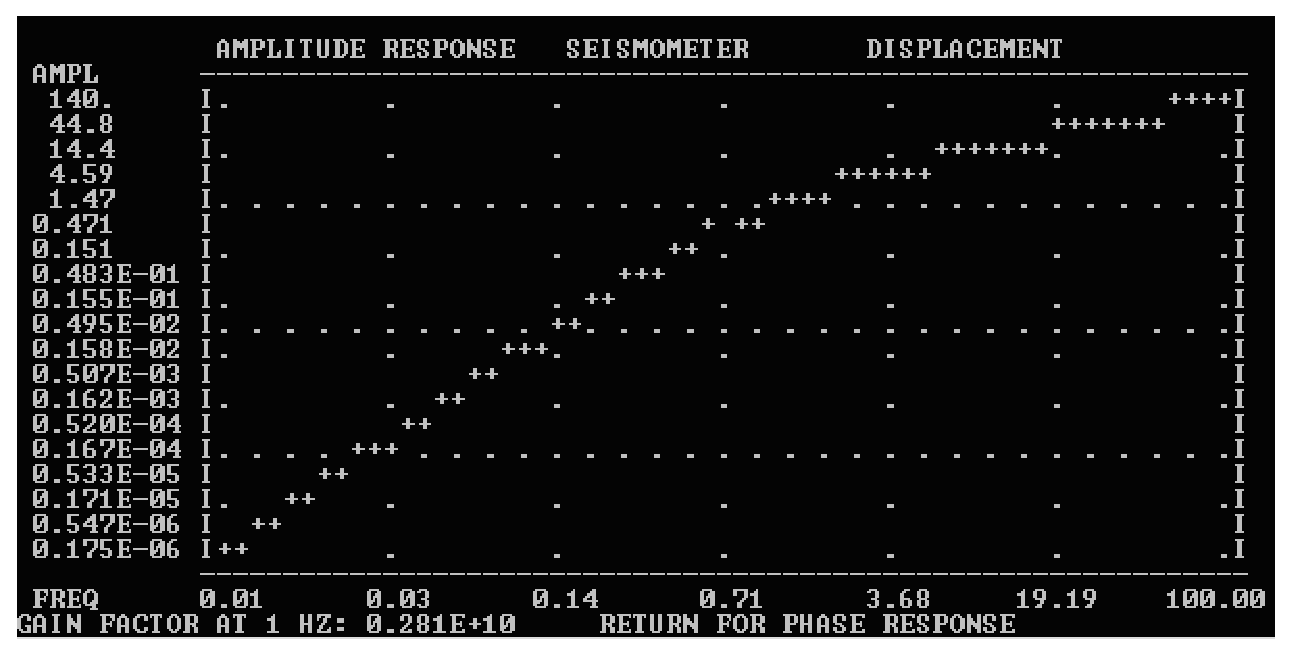
\includegraphics[width=0.9\linewidth]{fig/fig49}}
\caption{Making response file with parameters.}
%\label{fig:}
\end{figure}

\textbf{Making response file with poles and zeros}

The poles and zeroes velocity response in units of Hz is given as 

Poles \newline
-0.707 0.707 \newline
-0.707 -0.707 \newline
-62.4 135.4 \newline
-62.4 -135.4 \newline
-350.0 0.0 \newline
-75.0 0.0 

Zeros \newline
0.0 0.0 \newline
0.0 0.0 

SEISAN units are radians/sec so poles and zero values  are multiplied by $2\pi$. \newline
The normalization constant is given as $585.8 10^{6}$. To convert to radian is done as follows 

Normalization constant in radian = $585.8 10^{6} 2\pi^{(number of poles-number of zeroes)} 
= 585.8 10^{6} (2\pi)^{4} = 9.12 10^{11}$. 

SEISAN also uses displacement so one zero is added. The values are then 

Poles\newline
-4.442 4.442 \newline
-4.442 -4.442 \newline
-392.0 850.7 \newline
-392.0 -850.7 \newline
-2199.0 0.0 \newline
-475.0 0.0 

Zeros \newline
0.0 0.0 \newline
0.0 0.0 \newline
0.0 0.0 

To get total constant (gain and normalization constant),  we multiply by sensor gain and digitizer gain 

Total normalization constant = $9.12 10^{11} x 2002 x 312793 = 5.71 10^{20}$ 

A SEISAN input file is then made 

6 3 5.71e20 6 poles, 3 zeros and total gain constant \newline
-4.442 4.442 \newline
-4.442 -4.442 \newline
-392.0 850.7 \newline
-392.0 -850.7 \newline
-2199.0 0.0 \newline
-475.0 0.0 \newline
0.0 0.0 \newline
0.0 0.0 \newline
0.0 0.0 

The resp program now makes the SEISAN response file with this input as follows 

Output format: 0 Only testing \newline
Type of sensor: 0 Sensor response is in poles and zero file \newline
Recording media gain: 1 Gain has been put into total gain constant \newline
Amplifier gain: 0   No amplifier \newline
Number of filters: enter No filter \newline
File with poles and zeroes: \texttt{resp.inp} File with poles and zeros, can be any name \newline
File with tabulated values: enter \newline
File with measured values enter 

Then the plot below comes up 


\begin{figure}
\htmlimage{scale=2.0}
\centerline{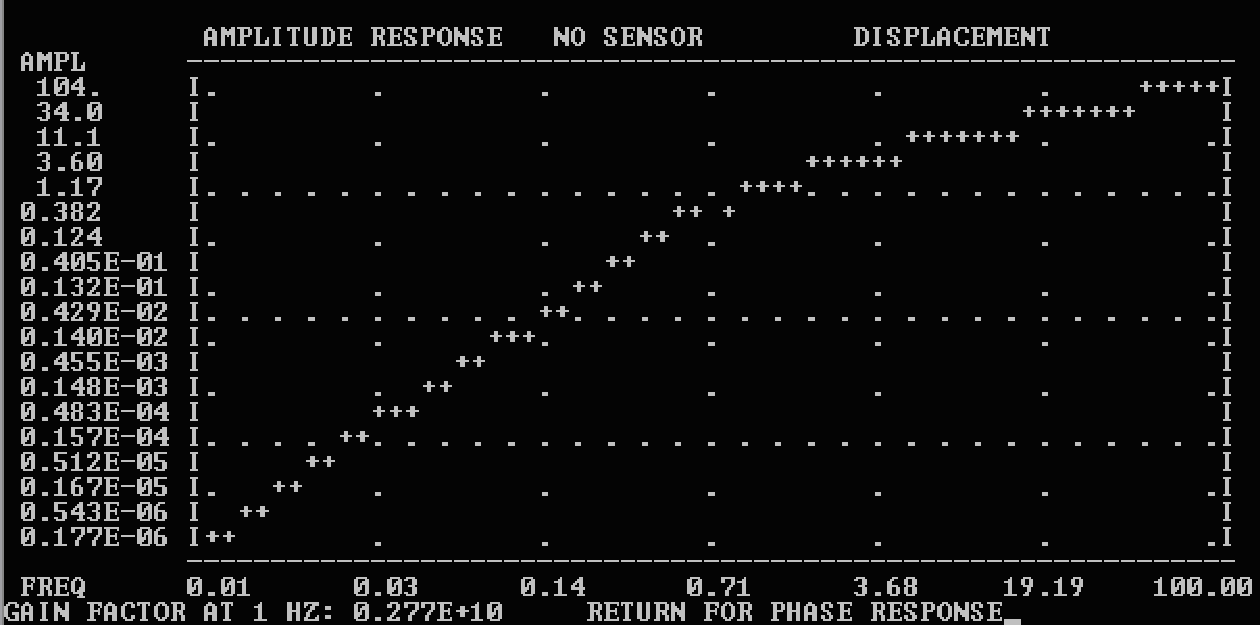
\includegraphics[width=0.9\linewidth]{fig/fig50}}
\caption{Making response file with poles and zeros.}
%\label{fig:}
\end{figure}

It is seen that the two ways of making the response file gives almost the same result, however using poles and zeroes is the most accurate, particularly for active sensors. In both cases no consideration was made for antialias filters which normally can be disregarded if a modern sharp filter. 

\textbf{Example of a Gurlp DM 24 digitizer with CMG-5T accelerometer}

The digitizer is the same as before 

Using parameter format, SEISAN currently requires the component name to start with A. According to international standards, the component code for an accelerometer should be something like ENZ so a parameter format cannot be used and poles and zeroes must be used. For the CMG-5T, the only information about the sensor is the sensitivity of 1V is equivalent to 0.970 m/s2 1.03 V/ms-1. In SEISAN parameter format this should be converted to V/g so sensitivity is then 

9.81 (ms-2/g)/0.97(ms-2/V) = 10.1 V/g  

\textbf{Parameter format}

The input is:  

Output format: 0  Only testing  \newline
Type of sensor: 3  It is an accelerometer  \newline
Generator constant: 10.1  \newline
Recording media gain: 312793  \newline
Amplifier gain: 0   No amplifier \newline
Number of filters: enter No filter \newline
File with poles and zeroes: enter We use parameters now \newline
File with tabulated values: enter \newline
File with measured values enter 

The plot below comes up 

\begin{figure}
\htmlimage{scale=2.0}
\centerline{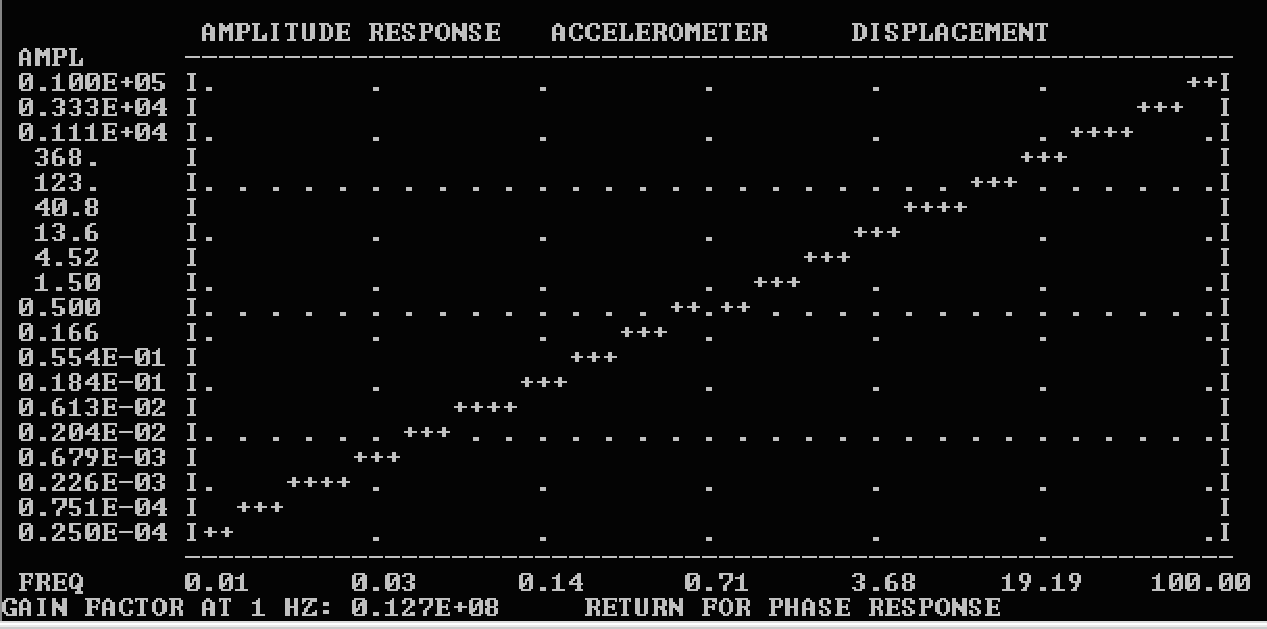
\includegraphics[width=0.9\linewidth]{fig/fig51}}
\caption{Making response file for an accelerometer woth parameters.}
%\label{fig:}
\end{figure}

\textbf{Poles and zeros}

The displacement response for an accelerometer consists of 2 zeros 
and normalizarion constant of 1. The total gain constant is then 

312793 x 1.03 = 322000 

So the input file for resp is 

0 2 322000\newline
0 0 \newline
0 0 

The manual input is exactly as above in the other example of using a poles and zero input file and the output is exactly as for the example of using parameter input. 

\textbf{Making a response file for a particular station}

For a particular station, chose output format SEISAN PAZ or GSE2 PAZ 
and later answering yes to question of making the SEISAN response 
file (see SEISAN manual ???????????????). 
If e.g. the station has station code TEST and component name S Z, 
the a response file valid from January 1, 2007 will have the name 
\texttt{TEST\_S\_\_Z.2007-01-00-0000\_SEI}. 
In case of a SEISAN poles and zero file, the content is:  

\verbatiminput{include/resp.sei}

So the file could have been made without using resp. 

Table 1 Example of \texttt{resp.out}: 

\verbatiminput{include/resp.out}

FOR MORE DETAILS ON HOW TO UNDERSTAND GSE AND SEED RESPONSE PARAMETERS, 
SEE \citep{havskov2004}, chapter 6. 

\subsection{SEED response} 


SEISAN can directly read SEED responses, which is poles and zeros, 
given as velocity response and transfer function types A (Laplace 
Transform in Rad/sec) and B (Analogue in 1/sec). Storage of response 
in one of these is the most common. The resp files can be created 
with rdseed from a full or dataless SEED volume 
(\texttt{rdseed -R -f seed\_volume}). RDSEED creates files with the 
pattern texttt{RESP.NC.STAT.LC.CHC}, where \texttt{NC}=network code, \texttt{STAT}=station code, 
\texttt{LC}=location code (not used by SEISAN) and \texttt{CHC}=channel code. The resp 
files need to be stored in the CAL directory and SEISAN will find 
the correct file. The resp file can contain response information from 
several time intervals. SEISAN uses the date and time of the waveform 
data to find the corresponding instrument response. 

SEED response files are given in stages, for example seismometer, digitizer and FIR filters are stored as individual stages. The overall response is made by combining all the stages. SEISAN uses the following blockets from the SEED resp file (for more details see \citet{iris1993}):

B052F22 - start date \newline
B052F23 - end date 

B053F03 - transfer function type, A=Laplace Transform (Rad/sec), B=Analog (1/sec) 

B053F07 - A0 normalization factor (A0 is checked against poles and zeros at normalization frequency and changed if not correct). The product of poles and zeros at the normalization frequency and A0 gives 1. 

B053F08 - Normalization frequency 

B053F10-13 - zeros, if transfer function type is B, normalization factor A0 is changed to (A0)/(2 pi) for each zero 

B053F15-18 - poles, if transfer function type is B, normalization factor A0 is changed to (A0)*(2 pi) for each pole 

B058F04 - gain 

The overall gain factor is given by the product of normalization factors and gain factors from all stages. One zero is added to convert to displacement response. It is assumed that input units are V/m and output units are counts, no checks are done on input and output units. 

\subsection{SEED response to GSE, SEEDRESP2GSE} 

SEEDRESP2GSE converts SEED resp files as written out by rdseed to GSE format. The program only supports poles and zeroes and transfer function type Laplace Transform. The program asks for station and component names and a time. This is because the resp file could have data from several channels and cover several time intervals with different instrument configuration. 

\subsection{GSE response to SEED, GSERESP2SEED} 

GSERESP2SEED can be used to build dataless SEED volumes from a set of 
GSE calibration files. The conversion is based on the GSE2SEED 
program by \textbf{Reinould Sleeman} (email sleeman@knmi.nl). Input can 
be single filenames or a list of files given in \texttt{filenr.lis}. The program produces a single channel SEED volume for each channel given by a GSE response file. At the end of the output filename, GSE is replaced by SEED. Other tools have to be used to merge several channels into one SEED volume. If there are several GSE files for a channel from different time periods, a stop date has to be given in the CAL2 line of the respective GSE file. Station coordinates are taken from the \texttt{STATION0.HYP} file. The program can use the site name, if it is part of the GSE response file through a comment line as in the following example: 

\begin{verbatim}
 (GSE2SEED_SITENAME Charnwood Forest, Leicestershire, England, UK) 
\end{verbatim}

